% !TEX root = ../main.tex

\chapter{Multigrid Methods}
\label{chapter:MultigridMethods}

\section{Smoothers}

% TODO: source Saad 2003

% TODO: define the linear problem Ax = b

% Quick comparison to direct
% TODO: fix the LU- QR- dash formatting if necessary.
For the solution of sparse linear systems, two distinct types of methods, iterative and direct methods, can be applied. For general purposes, direct methods usually utilize various decomposition or factorization techniques such as LU, QR, or Cholesky in order to achieve a solution to machine precision in a known finite amount of steps. The number of steps necessary for methods such as LU decomposition is shown by Saad~\cite{Saad2003} to be $O(n^3)$, which is increasingly disadvantageous for ever larger linear systems that are arising form the applicaiton of finite element methods.

% Advantages of relaxations: easy to implement, more general linear systems mgtut[23,24,26]
% (cf. Axelsson [6], Hackbusch [86], Varga [200])
Several variants of iterative methods exist, but for introducing and demonstrating the advantages multigrid methods, the focus will be on relaxation methods, such as Jacobi or Gauss-Seidel. These methods involve decomposition of the operator $A = D - L - U$ where $D$ is the diagonal of $A$, $-L$ is the strictly lower triangular part, and $-U$ is the strictly upper triangular part (cf. Saad~\cite{Saad2003}, Briggs et al.~\cite{Briggs2000}). The goal is then to use this decomposition to improve the starting guess $\mathbf{x}_{0}$, of the vector of unknowns $\mathbf{x}$ iteratively.

In the Jacobi scheme, rearranging after the decomposition of $A$ gives the iteration scheme

\begin{equation}
	\begin{aligned}
	\mathbf{x}^{(k+1)} &= D^{-1}(L + U)\mathbf{x}^{(k)} + D^{-1}\mathbf{b} \\
	                   &= R_J\mathbf{x}^{(k)} + D^{-1} \mathbf{b}
	\end{aligned}
\end{equation}

where matrix $R_J = D^{-1}(L + U)$ is defined as the Jacobi iteration matrix.

Component-wise, the updated $i$-th vector component can be obtained from the previous iteration's approximation of all other unknowns as:

\begin{equation}
	x_{i}^{(k+1)} = \frac{1}{a_{ii}}\left(b_i- \sum_{j \neq i}{a_{ij}x_{j}^{(k)}} \right).
\end{equation}

If the Jacobi method is initally used to compute an itermediate approximation, this can be weighted with a factor $\omega$ against the previous approximation, given in matrix form as

\begin{equation}
	\begin{aligned}
	\mathbf{x}^{(k+1)} &= \left[ (1-\omega) I + \omega R_J \right] \mathbf{x}^{(k)} + \omega D^{-1}\mathbf{b} \\
	&= R_{\omega}\mathbf{x}^{(k)} + \omega D^{-1} \mathbf{b}.
	\end{aligned}
\end{equation}

Different values of $\omega$ determines a factor known as the relaxtion rate which will be important to the idea of multigrid methods.

Similarly to the Jacobi method, the Gauss-Seidel method can be defined in the same manner, but with all already-updated individual vector components $1, 2, \ldots, j - 1$  being used in the approximation of the $j$-th component. This can be represented in matrix form as

\begin{equation}
	\begin{aligned}
	\mathbf{x}^{(k+1)} &= (D-L)^{-1}U\mathbf{x}^{(k)} + (D-L)^{-1}\mathbf{b} \\
                       &= R_G\mathbf{x}^{(k)} + (D-L)^{-1}\mathbf{b}
	\end{aligned}
\end{equation}

With $R_G = (D-L)^{-1}U$ defined as the Gauss-Seidel iteration matrix, the weighted version of the same method, known as Successive Over-Relaxation (SOR) is given as

\begin{equation}
	\mathbf{x}^{(k+1)} = (D - \omega L)^{-1} \left[(1-\omega)D + \omega U \right]\mathbf{x}^{(k)} + \omega (D - \omega L)^{-1} \mathbf{b}.
\end{equation}

% residual equation

% general form
The general form of these methods which rely on splitting of $A = M - N$ can be written as
\begin{equation}
	\mathbf{x}^{(k+1)} = M^{-1}N\mathbf{x}^{(k)} + M^{-1}\mathbf{b}
\end{equation}

and convergence of the iteration to the exact solution $\mathbf{x}^*$ can be obtained by examining the iteration in the form of and using the substitution $R = M^{-1}N $ :

\begin{equation}
	\mathbf{x^{(k+1)}} - \mathbf{x}^* = R\left(\mathbf{x}^{(k)} - \mathbf{x}^* \right) = \ldots = R^{k+1}\left(\mathbf{x}^{(0)} - \mathbf{x}^* \right).
\end{equation}

% \begin{equation}
% 	\mathbf{x^{(k+1)}} - \mathbf{x}^* = M^{-1}N\left(\mathbf{x}^{(k)} - \mathbf{x}^* \right) = \ldots = (M^{-1}N)^{k+1}\left(\mathbf{x}^{(0)} - \mathbf{x}^* \right).
% \end{equation}

The sequence can be shown to converge if and only if $\rho\left( R \right) < 1$. Without computing the spectral radius, which can be expensive, any matrix norm $|| R || < 1$ can be used as a sufficient convergence condition. For the Jacobi and Gauss-Seidel methods, it is also sufficient that $A$ is strictly or irreducibly diagonally dominant to converge for any $\mathbf{x}^{(0)}$, as is often the case with matrices obtained from the application of finite element methods. Additionally a strictly diagonally dominant matrix which is symmetric with positive diagonal entries is positive definite, and it is possible to show that for such SPD matrices Gauss-Seidel and SOR with $\omega \in (0, 2)$ will converge (cf. Saad~\cite{Saad2003}). %TODO cite Saad

% Disadvantages - Read Ch2

% Outline:
% + Direct vs Iterative
% 	+ operations
%  	- LU factorization fill-in
% + Different forms of Richardson, Jacobi, SOR.
% residual, error relationship
% general form of iteration/relaxation
% + damping
% + GS
% + convergence, spectral radius
% + smooth, fourier modes, wavenumbers (for certain matrices)
% + convergence rate of different error modes, smoothing property
%

\subsection{Smoothing Effect}

An examination of the effects of relaxation methods on the different error components is necessary to understand the motivation of multigrid methods. To show the effects of the relaxation methods on different error modes, as a concrete example, the weigted Jacobi method with $\omega = 2/3$ is used on the 1D Laplace equation with homogeneous Dirchlet boundary conditions is used as a model problem (cf. Trottenberg~\cite{Trottenberg2001}):

\begin{equation}
\begin{aligned}
	-\Delta_h u_h(x) &= 0, \quad x \in \Omega_h \\
	u_h(x) &= 0, \quad x \in \Omega_h.
\end{aligned}
\label{eq:model_problem}
\end{equation}

Where the problem is discretized on $\Omega = (0, 1) \subset \mathbb{R}$ with a grid spacing of $h = 1/n, n \in \mathbb{N}$ using a centered difference approximation stencil of $A = \frac{1}{h^2} \begin{pmatrix} -1 & 2 &-1 \end{pmatrix}$.

The eigenvectors $\mathbf{w}$ of $A$, equal to those of $R_{\omega}$ can be used in a linear combination to represent the error of the initial guess of the relaxation method $\mathbf{e}^{(0)}$

\begin{equation}
	\mathbf{e}^{(0)} = \sum_{k=1}^{n-1}{c_{k}\mathbf{w}_{k}}
\end{equation}

For the model problem, as shown by Briggs et al.~\cite{Briggs2000} the $j$-th component of each of these eigenvectors is given by
\begin{equation}
	w_{k,j} = sin\left(\frac{jk\pi}{n}\right),\ 1 \leq k \leq n-1,\ 0 \leq j \leq n
\end{equation}

These are also the Fourier modes, and are sine waves that increase in frequency with the wavenumber $k$. Repeated iteration of the relaxation scheme results in an eigenvector expansion for the error as

\begin{equation}
	\mathbf{e}^{(m)} = R_{\omega}^m \mathbf{e}^{(0)} = \sum_{k=1}^{n-1}{c_k\lambda_k^m\left( R_{\omega}\right)\mathbf{w}_k}.
\end{equation}

From this it can be seen that the error corresponding to the Fourier modes is reduced more for those error modes with a small corresponding eigenvalue $\lambda_k$. For this particular example, it can be shown that the eigenvalues are

\begin{equation}
	\lambda_k(R_{\omega}) = 1 - 2\omega sin^2\left(\frac{k\pi}{2n}\right),\ 1 \leq k \leq n-1,
\end{equation}

which is a monotonically decreasing function in $k$ with a maximum of 1 if $k = 0$ were allowed \cite{Briggs2000}. From this it can be inferred that although all error frequency components are reduced since $\lambda_k^m(R_{\omega}) < 1$ for all $k$, those with a low wavenumber $\left(k < \frac{n}{2}\right)$ and low frequency are reduced much more slowly due to the higher eigenvalue and these components will make up most of the error present after many iterations, while high-frequency $\left(k > \frac{n}{2}\right)$ error components will be much more effectively reduced. The error remaining will then be a combination of the low-frequency, or smooth, error modes, leading to this phenomenon being known as the \emph{smoothing effect}. For Gauss-Seidel iterations, although the eigenvectors of $R_G$ are not the same as $A$, Saad~\cite{Saad2003} shows this same smoothing effect after a more difficult analysis. The smoothing effect is not the end of the usefulness of the relaxation-based methods, and the multigrid method focuses on introducing corrections to these slowly converging smooth error components.

%TODO mention intuition for high-frequency error and stencil spatial relationship for the discretization

\section{Geometric Multigrid}

% - Coarse Grid Correction
% - interpolation, restriction
% - Two-grid scheme
% - V-Cycle, other cycles, FMG

\subsection{Prolongation and Restriction}

The key idea for overcoming the smoothing effect of relaxation schemes is to transfer the error to a coarser grid in which the low-frequency errors will appear to be more oscillatory, and relaxation methods would be more effective (\cite{Briggs2000}, \cite{Ruge1987}, \cite{Saad2003}). The error for the approximate solution $\mathbf{x}^{(k)}$ is given by

\begin{equation}
	\mathbf{e} = \mathbf{x}^* - \mathbf{x}^{(k)}.
\end{equation}

This error after several smoothing iterations is not known, but it is still useful to substitue into the equation for the residual for the given approximation $\mathbf{x}^{(k)}$, to obtain the \emph{residual equation} \cite{Briggs2000}:

\begin{equation}
	\begin{aligned}
	\mathbf{r} &= \mathbf{b} - A\mathbf{x}^{(k)} \\
	\mathbf{r} &= \mathbf{b} - A\left( \mathbf{x}^* - \mathbf{e} \right) \\
	\mathbf{r} &= A\mathbf{e}.
	\end{aligned}
\end{equation}

% TODO: talk a bit more about the P and R operators

Solving the residual equation for the error and correcting the approximation is another approach to solving the original problem, and this can be done after transferring the smooth error from a fine grid with $n_h$ points to a coarser grid with $n_H$ points by means of some linear operator, forming the basis of what is known as a two-grid correction scheme. For mapping the error from the fine grid $\Omega_h$ to the coarse grid $\Omega_H$, the restriction operator $R : \mathbb{R}^{n_h} \rightarrow \mathbb{R}^{n_H}$ is defined such that $\mathbf{e}_H = R_h \mathbf{e}_h$. The corresponding prolongation operator $P : \mathbb{R}^{n_H} \rightarrow \mathbb{R}^{n_h}$ is used to map from coarse to fine. This is often chosen to be $P = R^\top$, known as Galerkin coarsening. The error on the fine level can be approximated as

\begin{equation}
	\mathbf{e}_h \approx P_H \mathbf{e}_H,
\end{equation}

leading to

\begin{equation}
	\begin{aligned}
	\mathbf{r}_h & = A_h \mathbf{e}_h \approx A_h P_H \mathbf{e}_H \\
	\mathbf{r}_H & \approx R_h \mathbf{r}_h \approx R_h A_h P_H \mathbf{e}_H
	\end{aligned}
\end{equation}

where the product known as the Galerkin projection

\begin{equation}
	\label{eq:Galerkin}
	A_H := R_h A_h P_H
\end{equation}

can be used to represent the system matrix on the coarse grid. The Galerkin projection has the advantages of not needing to re-discretize the system on the coarser grid, turning this into an automatic process for black-box solvers, as well as avoiding unreliable sampling of system coefficients when the grid is too coarse~\cite{Wesseling2004}.
%^ Wesseling p 82

As a simple example for a one-dimensional coarse grid with $n_H = \frac{n_h}{2} - 1$, linear interpolation would result in a prolongation operator with the form

\begin{equation}
	P_H = \frac{1}{2}\begin{bmatrix}
		1 &   &   \\
		2 &   &   \\
		1 & 1 &   \\
		  & 2 &   \\
		  & 1 & 1 \\
		  &   & 2 \\
		  &   & 1
	\end{bmatrix}.
\end{equation}

The transpose of the linear interpolation $R_h = P_H^\top$ is known as full weighting. Due to aliasing effects after restriction, the high-frequency modes cannot be distinguished from lower-frequency modes, so the restriction should be used for an already-smoothed error.

\subsection{Two-Grid Correction Scheme}

This leads to the formation of the two-grid correction scheme shown in Algorithm~\ref{alg:two_grid}. With an inital starting guess $\mathbf{x}_h$, relaxation can be done a total of $\nu_1$ times until the error is sufficiently smooth and improvements in the approxmation would be slow. The residual is then restricted to the coarse grid $\Omega_H$, in order to represent smooth error components as more oscillatory, and the residual equation is solved for the error $\mathbf{e}_H$ on the coarse grid. Solving for the error can be done with any number of methods, such as exactly with a direct solver. An approximate solution is also possible, for example, with another grid correction scheme, which will be discussed in the following section. The error can be prolongated back to the fine grid $\Omega_h$ and used to correct the fine-grid approximation. The prolongated error is not necessarily as smooth as on the coarse grid, so $\nu_2$ post-smoothing steps are performed.

%Wesseling pg. 12
One of the most important properties of this two grid scheme is that the convergence rate can be shown to be independent of the grid spacing $h$. This is not the case for the smoothers which they are based on, whose convergence behaves as $1 - O(h^2)$~\cite{Wesseling2004}. This is because decreasing the grid spacing for the previously discussed smoothers increases the eigenvalues of the error modes with the lowest wavenumbers, resulting in even slower convergence for the corresponding smooth components of the error.

\begin{algorithm}
	\caption{Two-Grid Correction Scheme}\label{alg:two_grid}
	\begin{algorithmic}[1]
		\Require{Fine-level system $A_h$ and $\mathbf{b}_h$}
		\Require{Initial guess $\mathbf{x}_h$}
		\Require{Number of pre- and post-smoothing steps $\nu_1$ and $\nu_2$}
        \Procedure{Two-Grid-Correction}{$A_h, \mathbf{x}_h, \mathbf{b}_h$}
		\For{$k \gets 1, \nu_1$}
			\State $\mathbf{x}_h \gets \Call{smoother}{A_h, \mathbf{x}_h, \mathbf{b}_h}$ \Comment{Apply $\nu_1$ pre-smoothing steps}
		\EndFor
		\State $\mathbf{r}_h \gets \mathbf{b}_h - A_h \mathbf{x}_h$ \Comment{Compute residual on fine grid}
		\State $\mathbf{r}_H \gets R \mathbf{r}_h$ \Comment{Restrict residual to coarse grid}
		\State Solve $A_H \mathbf{e}_H = \mathbf{r}_H$ \Comment{Solve residual equation on coarse grid $\Omega_H$} \label{alg:two_grid_solve}
		\State $\mathbf{e}_h \gets P \mathbf{e}_H$ \Comment{Prolongate coarse-grid error to fine grid}
		\State $\mathbf{x}_h \gets \mathbf{x}_h + \mathbf{e}_h$ \Comment{Correct fine grid approximation $\mathbf{x}_h$}
		\For{$k \gets 1, \nu_2$}
			\State $\mathbf{x}_h \gets \Call{smoother}{A_h, \mathbf{x}_h, \mathbf{b}_h}$ \Comment{Apply $\nu_2$ post-smoothing steps}
		\EndFor
		\EndProcedure
	\end{algorithmic}
\end{algorithm}

\subsection{Multiple Grids}

A natural progression is to not require an exact solution to the coarse-grid problem in Algorithm~\ref{alg:two_grid} line \ref{alg:two_grid_solve}, but instead recursively use the two-grid scheme on an even coarser grid. When some coarsest grid is reached, the problem will be small enough to quickly solve.

%TODO: should it be L-1 levels?
Using $L + 1$ increasingly coarser grids, $\Omega_{h_0}, \ldots, \Omega_{h_{\ell}}, \ldots, \Omega_{h_{L-1}}, \Omega_{h_L}$, the restriction and prolongation operators an be defined in accordance with which levels they map between: $I_{\ell-1}^\ell$ for restriction and $I_\ell^{\ell-1}$ for prolongation. Starting from the finest grid, the two-grid cycle can be performed recursively to refine the error. The amount of times the recursion is called at a particular level can be chosen with a paramter $\gamma$. This will result in a particular pattern through which the algorithm tranfers between grids. With $\gamma = 1$ a V-cycle is obtained, and with $\gamma = 2$ a W-cycle is obtained. This is detailed in Algorithm~\ref{alg:multigrid}.

% Define algorithm
\begin{algorithm}
	\caption{Multigrid}\label{alg:multigrid}
	\begin{algorithmic}[1]
		\Procedure{Multigrid}{$A_\ell, \mathbf{x}_\ell, \mathbf{b}_\ell$}
		\For{$k \gets 1, \nu_1$}
			\State $\mathbf{x}_\ell \gets \Call{smoother}{A_\ell, \mathbf{x}_\ell, \mathbf{b}_\ell}$ \Comment{Apply $\nu_1$ pre-smoothing steps}
		\EndFor

		\If{$\ell = L$}
			\State Solve $A_\ell \mathbf{x}_\ell = \mathbf{b}_\ell$ \Comment{Solve equation on coarsest grid $\Omega_{h_L}$}
			\State \textbf{return} $x_\ell$
		\Else
			\State $\mathbf{r}_\ell \gets \mathbf{b}_\ell - A_\ell \mathbf{x}_\ell$ \Comment{Compute residual on fine grid}
			\State $\mathbf{r}_{\ell+1} \gets I_{\ell}^{\ell + 1} \mathbf{r}_\ell$ \Comment{Restrict residual to coarse grid}
			\State $\mathbf{e}_{\ell+1} \gets 0$
			\For{$k \gets 1, \gamma$}
				\State $\mathbf{e}_{\ell+1} \gets \Call{Multigrid}{A_{\ell+1}, \mathbf{e}_{\ell+1}, \mathbf{r}_{\ell+1}}$ \Comment{Perform recursion $\gamma$ times}
			\EndFor
			\State $\mathbf{e}_{\ell} \gets I_{\ell + 1}^{\ell} \mathbf{e}_{\ell+1}$ \Comment{Prolongate coarse-grid error to fine grid}
			\State $\mathbf{x}_{\ell} \gets \mathbf{x}_{\ell} + \mathbf{e}_{\ell}$ \Comment{Correct fine grid approximation $\mathbf{x}_{\ell}$}
		\EndIf

		\For{$k \gets 1, \nu_2$}
			\State $\mathbf{x}_\ell \gets \Call{smoother}{A_\ell, \mathbf{x}_\ell, \mathbf{b}_\ell}$ \Comment{Apply $\nu_2$ post-smoothing steps}
		\EndFor
		\State \textbf{return} $x_\ell$
		\EndProcedure
	\end{algorithmic}
\end{algorithm}

% V, W, Full cyclce

% brief overview of convergence, computational work?


\section{Algebraic Multigrid}

% Talk a bit more and mention primary sources as a general citation

On an unstructured grid, the geometric approach cannot be applied as the formulation is dependent on the locations of the nodes of the grid. For a grid where the locations of the grid nodes are unknown, where they are unstructured, or where an arbitrary system of equations does not refer to a physical grid, an algebraic multrigrid (AMG) method can be used instead. Instead of relying on information about the geometry of the discretization, only information from the matrix $A$ is used to determine the prolongation and restriction operators. AMG methods are shown in depth by Ruge~\cite{Ruge1987}, Briggs et al.~\cite{Briggs2000}, Falgout~\cite{Falgout2006}, and Stüben~\cite{Stuben1999}.

\subsection{Algebraically Smooth Error}

For algebraic multigrid, the general idea starts the same with choosing a subset of unknowns for coarsening. Similar to selecting a coarse grid in multigrid, the smooth error modes should be transfered to a coarse grid which accurately represents them, but this coarse grid must be defined algebraically.

In the geometric case, the dominant error components after relaxation have low frequencies and are considered to be smooth. This concept of smoothness can be generalized to the algebraic case by considering the algebraically smooth error to be any error which is slowly reduced by the relaxation method, which then must be corrected on the coarser levels, i.e. an error for which $ \|(I - R^{-1}A)\mathbf{e}^{(k)}\|_A \approx \| \mathbf{e}^{(k+1)}\|_A $.

For relaxation schemes such as Jacobi, Gauss-Seidel, as well as their weighted variants, the smooth error is characterized by $ A\mathbf{e} \approx 0 $. Additionally, error components considered to be "smooth" can be more precisely defined as having a small residual comparable to the error. These smooth errors are the eigenvectors with the smallest eigenvalues and are in the near null space of $A$. These modes are damped the least by the relaxation scheme, so the coarse level correction should be effective for this error (\cite{Falgout2006}, \cite{Ruge1987}).
%falgout-2006 amg - "near null space important" pg 4 as well as ruge1987

It is shown in Stüben~\cite{Stuben1999} for algebraically smooth error of symmetric M-matrices, the following holds:

\begin{equation}
	\sum_{i \neq j}{\frac{|a_{ij}|}{a_{ii}}\frac{(e_i - e_j)^2}{e_i^2}} \ll 1,\ 1 \leq i \leq n.
	\label{eq:strong_connection}
\end{equation}

This can be interpreted as such: if the first term is large, implying that the off-diagonal element is comparable to the diagonal element, then $e_i - e_j$ must be small, or in other words, the smooth error must vary slowly from $e_i$ to $e_j$. For two unknowns, a relatively large coefficient $a_{ij}$ means that $u_j$ has an important influence in determining $u_i$, meaning that the point $u_i$ has a strong dependence on $u_j$. Conversely $u_j$ is said to have a strong influence on $u_i$. To be specific about a the strength of the influence, Falgout~\cite{Falgout2006} gives the definition of the \emph{strength of connection}: Given a threshold $0 < \theta \leq 1$, $u_i$ \emph{strongly depends} on variable $u_j$ if

\begin{equation}
-a_{ij} \geq \theta \max_{k \neq i}{\{-a_{ik}\}}.
\label{eq:strong_connection2}
\end{equation}

\subsection{Interpolation Operator} %TODO: rename

For the coarse grid, a subset of points need to be chosen such that the grid is coarsened in the direction on strong connections. Strong connections indicate slowly varying smooth error, as above, which make such strongly connected points good candiates to accurately interpolate from a coarse to fine grid. This idea will be used to construct an interpolation operator $I_{2h}^h$ for a coarse grid, the selection of which will be explained in the following section. The indices can be partitioned into two sets, $C$ and $F$. The set $C$ is defined as the points corresponding coarse-grid points, also present on the fine grid. The set $F$ is correspoints to points that are only present on the fine grid. To interpolate error $e_i, i \in C$ to the fine grid $C \cup F$, the points not present in C are a weighted average:

% TODO definition of "neighborhood" of i
% TODO: change all h & 2h's
\begin{equation}
	(I_{2h}^h\mathbf{e})_i =
		\begin{cases}
			e_i & \text{if $i \in C$,} \\
			\displaystyle \sum_{j \in C_i}{w_{ij}e_j} & \text{if $i \in F$,}
		\end{cases}
	\label{eq:interpolation_operator}
\end{equation}

For determining the weights $w_{ij}$, the smooth error is characterized by its small residual $r = A\mathbf{e} \approx 0$, with one component of the residual being $r_i = \sum_{j}{a_{ij}e_j} = 0$. The only points to be concerned with are points in the \emph{neighborhood of i} $N_i$, which are the points that even have connection to point $i$, i.e. $a_{ij} \neq 0$. Defining $S_i$ as the set of all strong connections to point $i$, the residual can be reformulated by considering three types of neighboring points to $i$ (cf. \cite{Briggs2000}):
\begin{enumerate}
	\item The set $C_i$ of C-points which strongly influence $i$, $C_i = C \cap S_i$, also called the \emph{coarse interpolatory set}
	\item The set $D_i^s$ of F-points which strongly influence $i$, with $D_i = N_i - C_i$, and $D_i^s = D_i \cap S_i$, called strong noninterpolatory connections
	\item The set $D_i^w$ of F-points which do not strongly influence $i$, $D_i^w = D_i - S_i$, called weak noninterpolatory connections
\end{enumerate}

The sum can then be regrouped in terms of point $i$ and the three sets $C_i$, $D_i^s$, and $D_i^w$:

\begin{equation}
	a_{ii}e_i \approx -\sum_{j \in C_i}{a_{ij}e_j} - \sum_{j \in D_i^s}{a_{ij}e_j} - \sum_{j \in D_i^w}{a_{ij}e_j}
\end{equation}

% TODO: elaborate why these approx can be made
For points $j \in D_i^w$, $e_j$ can be grouped with $e_i$ and points in $D_i^s$ can be approximated by

\begin{equation}
	e_j \approx \frac{\displaystyle \sum_{k \in C_i}{a_{jk}e_k}}{\displaystyle \sum_{k \in C_i}{a_{jk}}}.
	\label{ej_approx}
\end{equation}

Then the weights can be represented by

\begin{equation}
	w_{ij} = - \frac{a_{ij} + \displaystyle \sum_{m \in D_i^s}{\left(\frac{a_{im}a_{mj}}{\displaystyle \sum_{k \in C_i}{a_{mk}}}\right)}}{a_{ii} + \displaystyle \sum_{n \in D_i^w}{a_{in}}}
\end{equation}

\subsection{Coarse Grid} %TODO: rename

Now that the interpolation operator has been defined, it is now necessary to determine which points will be in the coarse interpolatory set for each point on the fine grid. These points will make up the coarse grid. The approximation made in Equation~\ref{ej_approx} is more accurate the more strongly connected $j$ is to $i$, so this can be used as a heuristic criterion for choosing the coarse grid points. Another criterion is necessary to also limit the size of the coarse set. These two criteria are given by Ruge and Stüben~\cite{Ruge1987} as:

\begin{itemize}
	\item (C1) For each $i \in F$, each point $j \in S_i$ should either be in $c$, or should be strongly connected to at least one point in $C_i$.
	\item (C2) $C$ should be a maximal subset of all points with the property that no two C-points are strongly connected to each other.
\end{itemize}

% explanation on why C2 is needed: it strikes a balance on the size of the coarse grid, whihc should be a small fraction of the total points to reduce the work per cycle.
The criterion (C2) is motivated by limiting the amount of numerical work done on the coarse grid, since no two C-points being directly connected will lead to a lesser amount of coarse grid points. In some situations both of these criteria cannot be fulfilled, so (C1) is considered to be necessary, while (C2) is used as a guideline to achieve (C1).

The coarsening process which adheres to the two criteria is a two-pass algorithm. The first pass is a quick preliminary partition of the grid into $C$- and $F$-points, while ensuring (C2) as well as possible. The second part consists of computing the weights for the interpolation operator while changing any intial $F$-points to $C$-points in order to satisfy (C1).

The entire algorithm presented is highly dependent on a proper choice of $\theta$ in Equation~\ref{eq:strong_connection2}. Falgout~\cite{Falgout2006} noted that an improper choice could lead to slower performance due to too many points being considered strong connections and resulting in too large of a coarse grid.

\section{Smoothed Aggregation Algebraic Multigrid}
% TODO: cite Vanek
Smoothed aggregation algebraic multigrid (SA-AMG) is a type of algebraic multigrid method which groups nodes together into aggregates to form the coarse-level problem, as opposed to including individual nodes in the fine- and coarse-grid sets. Similarly to AMG, forming these aggregates uses only algebraic information present in $A$, and the problem does not necessarily need to be represented on a geometric grid. Aggregation-based multigrid methods have a different set of requirements for forming the prolongation operators, which are discussed in Van\v{e}k~(\cite{Vanek1996},~\cite{Vanek1996_unstruc}) and Mandel~\cite{Mandel1999}. The tentative prolongation operators are chosen by an aggregation method which results in operators that meet these requirements. These tentative operators are then finally smoothed in order to decrease the energy of the coarse level basis functions. The requirements that the prolongation operators should satisfy are (cf. \cite{Vanek1996_unstruc}):

\begin{itemize}
	\item (AMG1) \textbf{Supports of coarse basis functions follow strong couplings.} Two nodes $i$ and $j$ are strongly coupled if the matrix coefficient $|a_{ij}|$ is large relative to $\sqrt{|a_{ii}a_{jj}|}$. This requirement is motivated for anisotropic problems so that semi-coarsening is achieved in the direction of anisotropy, meaning that coarse basis functions should be supported by strongly coupled nodes.
	\item (AMG2) \textbf{Bounded intersection.} On a given level the support of each coarse basis function should intersect only a bounded number of supports of other basis functions. For a given bound on the number of intersecting supports $K$, the number of nonzeroes in $A_\ell$ is bounded by $K+1$, thus guaranteeing that the coarse level matrices remain sufficiently sparse to reduce computational costs.
	\item (AMG3) \textbf{Coarse space contains zero energy modes.} This involves preserving the kernel or null space on the coarse levels, which for elasticity is the rigid body translations and rotations. Similar to AMG, the motivation for this is to replace the notion of geometrically smooth error for aggregation methods, where the smooth error components are characterized by a small residual, i.e $A_\ell\mathbf{e} \approx 0$, and should be transfered to the coarse grid, so the prolongator should accurately interpolate these modes.
	\item (AMG4) \textbf{Small Energy.} The energy of each coarse basis function should be minimal so that condition number of the resulting operators is small, and to avoid transfering oscillatory error components to the coarse level \cite{Mandel1999}.
	\item (AMG5) \textbf{Uniform $L^2$ equivalence.} The discrete $l^2$ and continuous $L^2$ norms should be equivalent on all coarse spaces.
\end{itemize}

\subsection{Aggregation}
The aggregation algorithm can be broken up into three parts, a first-pass aggregation, expansion of existing aggregate sets, and clean-up any remnants that may exist. A basic general form of aggregation is described in this section, but other aggregation algorithms exist for more specialized purposes. The idea of strong connections from AMG are combined with the neighborhood to define the strongly-coupled neighborhood for node $i$ on level $\ell$,

\begin{equation}
	\label{eq:strong_neighborhood}
	N_i^\ell = \left\{ j : |a_{ij}| \geq \varepsilon \sqrt{|a_{ii} a_{jj} |} \right\} \cup \left\{ i \right\},
\end{equation}

where $\varepsilon > 0$ is chosen to adjust the strength of couplings included in the set. Especially for anisotropic problems, the coarse basis functions should follow the direction of strong couplings, so choosing aggregates consisting of a strongly-coupled neighborhood helps to satisfy requirement (AMG1). Algorithm~\ref{alg:aggregation} outlines the aggregation procedure introduced by Van\v{e}k~\cite{Vanek1996_unstruc} to group the nodes into aggregate sets which form a disjoint covering $\{C_i^\ell\}_{i=1}^{n_\ell + 1}$ of the set of nodes.

Step 1 of the aggregation process attempts to cover as much of the nodes as possible with strongly copuled neighborhoods. However, an unaggregated node after this step could still contain part or all of its strongly-coupled neighborhood in other aggregates, and thus would be ignored as a part of a disjoint covering. Different coverings are possible depending on the order in which the neighborhoods are considered. Some more specialized algorithms introduce minimum and maximum sizes for aggregates. One advantage of specifying this is to make the aggregate sizes more uniform. Additionally, the optimal size of aggregates in each dimension is 3, such that that the system matrix on the next level which are constructed from these aggregates are not too dense due to the overlapping of the coarse basis functions.

Step 2 of the aggregation checks if each remaining unaggregated node is strongly coupled to another aggregate, and then expands that aggregate to include the node. It is usually the case that these unaggregated nodes exist, because they are not directly in neighborhood as defined by a node $i$ in equation~\ref{eq:strong_neighborhood}, but still share nodes that are strongly coupled to both.

In step 3 any still unaggregated nodes are grouped into a new aggregate with any nodes in their neighborhood which are also unaggregated. This can happen if the node is too isolated such that there is no strongly coupled connection to existing aggregates step 2. Overall, one consideration is that for many systems, such as elasticity problems, each node has multiple degrees of freedom. The aggregation algorithm should take into account that multiple degrees of freedom in the system matrix $A$ should be considered to be a part of one node, even when the nodes are not defined on a geometric grid.

An example of this aggregation process is shown in figure~\ref{fig:aggregation_example}. On this example, the order in which the nodes were iterated through determined the distribution of aggregates after step 1. It is also possible that for a larger grid, the aggregates could be more tightly packed after step 1 if the nodes were considered in a different order.

\begin{algorithm}
	\caption{Aggregation}\label{alg:aggregation}
	\begin{algorithmic}[1]
		\Procedure{Aggregation}{$A^\ell$}
			\Statex \textbf{Step 1: First-pass aggregation}
			\State $R \gets \{ i \in 1, \ldots, n_l\}$ \Comment{Initialize the set of unaggregated nodes}
			\State $C \gets \emptyset$ \Comment{Initialize set of aggregates}
			\State $j \gets 0$ \Comment{Number of aggregates}
			\ForAll{$i \in R$}
				\If{$N_i^\ell \subset R$}
					\State $j \gets j+1$
					\State $C_j^\ell \gets N_i^\ell$ \Comment{Group strongly coupled neighborhood of $i$ into an aggregate}
					\State $R \gets R \setminus C_j^\ell$ \Comment{Remove from unaggregated nodes}
				\EndIf
			\EndFor \Comment{R can still contain unaggregated subsets of neighborhoods}
			\Statex
			\Statex \textbf{Step 2: Expand existing aggregates}
			\For{$k \gets 1, j$}
				\State $\tilde{C}_k^\ell \gets C_k^\ell$
			\EndFor
			\ForAll{$i \in R$} \Comment{For all unaggregated nodes in first pass}
				\If{$\exists k \ni N_i^\ell \cap \tilde{C}_k^\ell \neq \emptyset$} \Comment{Exists aggregate sharing part of the neighborhood?}
					\State $C_k^\ell \gets C_k^\ell \cup \{ i \}$ \Comment{Enlarge the existing aggregate}
					\State $R \gets R \setminus \{ i \} $
				\EndIf
			\EndFor
			\Statex
			\Statex \textbf{Step 3: Aggregate remnants}
			\ForAll{$i \in R$} \Comment{$R$ is remnants which were not aggregated}
				\State $j \gets j + 1$
				\State $C_j^\ell \gets R \cap N_i^\ell$ \Comment{Group only unaggregated nodes from the neighborhood}
				\State $R \gets R \setminus C_j^\ell$
			\EndFor
		\EndProcedure
	\end{algorithmic}
\end{algorithm}

\begin{figure}
\centering
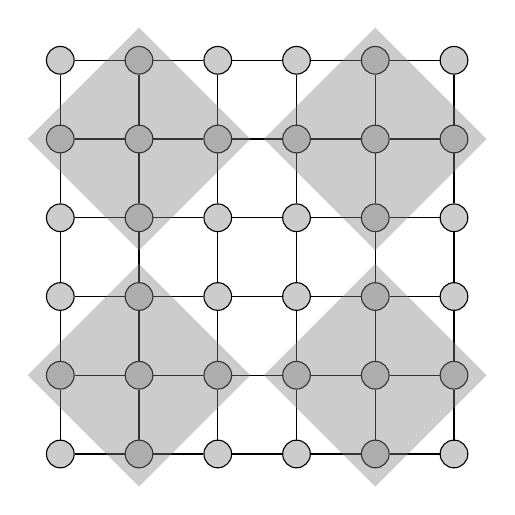
\begin{tikzpicture}[darkstyle/.style={circle,draw,fill=gray!40,minimum size=10}]
	\foreach \x in {0,...,5}
	  \foreach \y in {0,...,5}
		 {\pgfmathtruncatemacro{\label}{\x - 5 *  \y +21}
		%  \node [darkstyle]  (\x\y) at (1.5*\x,1.5*\y) {};}
		 \node [darkstyle]  (\x\y) at (\x,\y) {};}

	\foreach \x in {0,...,5}
	  \foreach \y [count=\yi] in {0,...,4}
		\draw (\x\y)--(\x\yi) (\y\x)--(\yi\x) ;
	\fill[gray,opacity=0.4,cm={cos(45) ,-sin(45) ,sin(45) ,cos(45) ,(1 cm,4 cm)}] (1,1) -- (1,-1) -- (-1,-1) -- (-1,1) -- (1,1);
	\fill[gray,opacity=0.4,cm={cos(45) ,-sin(45) ,sin(45) ,cos(45) ,(4 cm,4 cm)}] (1,1) -- (1,-1) -- (-1,-1) -- (-1,1) -- (1,1);
	\fill[gray,opacity=0.4,cm={cos(45) ,-sin(45) ,sin(45) ,cos(45) ,(1 cm,1 cm)}] (1,1) -- (1,-1) -- (-1,-1) -- (-1,1) -- (1,1);
	\fill[gray,opacity=0.4,cm={cos(45) ,-sin(45) ,sin(45) ,cos(45) ,(4 cm,1 cm)}] (1,1) -- (1,-1) -- (-1,-1) -- (-1,1) -- (1,1);

  \end{tikzpicture}\hspace{1cm}%
  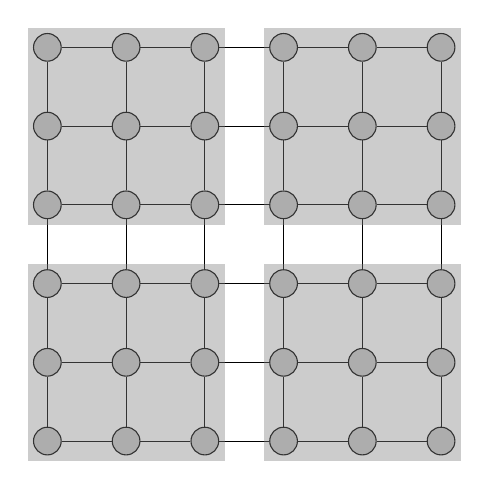
\begin{tikzpicture}[darkstyle/.style={circle,draw,fill=gray!40,minimum size=10}]
	\foreach \x in {0,...,5}
	  \foreach \y in {0,...,5}
		 {\pgfmathtruncatemacro{\label}{\x - 5 *  \y +21}
		%  \node [darkstyle]  (\x\y) at (1.5*\x,1.5*\y) {};}
		 \node [darkstyle]  (\x\y) at (\x,\y) {};}

	\foreach \x in {0,...,5}
	  \foreach \y [count=\yi] in {0,...,4}
		\draw (\x\y)--(\x\yi) (\y\x)--(\yi\x) ;
		\fill[gray,opacity=0.4] (-0.25,-0.25) rectangle (2.25, 2.25);
		\fill[gray,opacity=0.4] (5.25,-0.25) rectangle (2.75, 2.25);
		\fill[gray,opacity=0.4] (5.25, 5.25) rectangle (2.75, 2.75);
		\fill[gray,opacity=0.4] (-0.25, 5.25) rectangle (2.25, 2.75);

  \end{tikzpicture}
  \caption{An example of the aggregation process for a graph where the strongly coupled nodes are in the pattern of a 5-point stencil. On the left, the nodes which have been aggregated after step 1 of the aggregation are shaded. At this step, there are no more nodes with a completely unaggregated strongly coupled neighborhood. On the right, the existing aggregates are expanded according to step 2. After this there are no more unaggregated nodes, so step 3 of the aggregation process is unnecessary.}
  \label{fig:aggregation_example}
\end{figure}

\subsection{Prolongation Operators}

Once the degrees of freedom on a level have been aggregated, if the problem is scalar, one choice for a tentative prolongation operator $\tilde{P}_\ell$ is to simply use

\begin{equation}
	\left(\tilde P_\ell \right)_{ij} =
	\begin{cases}
		1 & \text{if $i \in C_j^\ell$}, \\
		0 & \text{otherwise}.
	\end{cases}
\end{equation}

This is insufficient for systems of equations, such as elasticity problems, where this tentative prolongator has to be formed by minimizing the energy in order to sastisy constraint (AMG3). This needs to be done by using the aggregates to define the sparsity pattern of $\tilde{P}_\ell$ while ensuring that near null space modes are transfered to the coarse level to be eliminated. For elasticity, on the finest level the null space dimension $n_{ns}$ is 3 in two dimensions, and 6 in three dimensions, consisting of the rigid body translations and rotations \cite{Gee2009}. The near null space $B_\ell \in \mathbb{R}^{n_\ell \times n_{ns}}$ satisfies $\tilde{A}_\ell B_\ell = 0$, where $\tilde{A}$ is the stiffness matrix without Dirichlet boundary conditions. Starting from the finest level, both the tentative prolongators as well the coarse near null space vectors can then be constructed at each level $\ell = 1, \ldots, L - 1$ by satisfying
% slow converging smooth error modes need to be minimized. Mandel 1999

\begin{equation}
	\label{eq:prolongator_req}
	\begin{aligned}
	& B_\ell = \tilde{P}_\ell B_{\ell+1} \\
	& \tilde{P}_\ell^\top \tilde{P}_\ell = I
	\end{aligned}
\end{equation}

This can be done through the process shown by Mandel et al.~\cite{Mandel1999} starting with partitioning $B_\ell$ into $m$ sets of rows $B_\ell^k,\ k = 1, \ldots, m$ so that each set of rows corresponds to an aggregate. Because of the requirement that $P_\ell$ is orthogonal, a QR-decomposition is performed on each set $B_\ell^{k} = Q_\ell^k R_\ell^k$, where $Q_\ell^k \in \mathbb{R}^{n_k \times n_{ns}}$ is orthogonal and $R_\ell^k \in \mathbb{R}^{n_{ns} \times n_{ns}}$ is an upper triangular square matrix. Afterwards the individual $R_\ell^k$ matrices can be combined back as blocks to form $B_{\ell+1}$
\begin{equation}
	B_{\ell+1} =
	\begin{pmatrix}
		R_\ell^1 \\
		R_\ell^2 \\
		\vdots \\
		R_\ell^m
	\end{pmatrix}.
\end{equation}
The resulting $Q_\ell^k$ matrices are combined in a block diagonal matrix to form the prologator of the current level:
\begin{equation}
	\tilde{P}_\ell = \text{diag}\left(Q_\ell^1, \ldots, Q_\ell^m\right) =
	\begin{pmatrix}
		Q_\ell^1 &          &        & \\
		         & Q_\ell^2 &        & \\
				 &          & \ddots & \\
				 &          &        & Q_\ell^m
	\end{pmatrix}.
\end{equation}
Because of the way that $B_\ell$ is initially partitioned into sets corresponding to aggregates, the sparsity pattern of $\tilde{P}_\ell$ is determined by the aggregates. It has a block diagonal structure, so the aggregates being a disjoint covering of the nodes helps to ensure the requirement (AMG2). A consideration for 3D elasticity problems in Van\v{e}k~\cite{Vanek1996} is that the finest level has 3 degrees of freedom per node, but with 6 rigid body modes, the coarser levels have 6 degrees of freedom per node. Then if an aggregate does not contain two or more nodes, some of the tentative basis functions can be linearly dependent. This can be avoided in the aggregation process by disallowing single node aggregates.

\subsection{Smoothing Prolongators}

After the tentative prolongators have been constructed for each level, the energy of the discrete coarse basis functions corresponding to the columns of $\tilde{P}_\ell$ can be further reduced by smoothing to obtain the final prolongator $P_\ell$. This further improves the condition number at coarser levels and prevents oscillatory error modes from being transfered. As a simple choice the weighted Jacobi smoother can be used resulting in

\begin{equation}
	\label{eq:P_smoothing}
	P_\ell = (I - \omega D^{-1}A_\ell)\tilde{P}_\ell.
\end{equation}

The smoothing will worsen the requirement (AMG2) by causing some overlap in the basis functions, but will improve requirement (AMG4) by reducing the energy. For anisotropic problems, the matrix used in smoothing can be filtered first to decrease the number of non-zeros as well as to improve coarsening in the direction of strong couplings (\cite{Gee2009}, \cite{Vanek1996}). The filtered matrix can be defined as $A_\ell^F = \left(a_{ij}^F\right)$ where
\begin{equation}
	\begin{aligned}
	a_{ij}^F &=
	\begin{cases}
		a_{ij} & \text{if $j \in N_i^\ell$} \\
		0 & \text{otherwise}
	\end{cases}, \text{if $i \neq j$}, \\
	a_{ii}^F & =  a_{ii} - \displaystyle \sum_{j=1, j\neq i}^{n_\ell}{\left(a_{ij} - a_{ij}^F\right)}.
	\end{aligned}
\end{equation}

After smoothing is complete, the remaining part of the process is to define the coarse-level problem on the next level $A_{\ell+1}$, after which the process can repeat until a maximum number of levels is reached or a sufficiently small coarse level problem is achieved. Once again, the Galerkin projection defined in equation~\ref{eq:Galerkin} with $R = P^\top$ can be used to define

\begin{equation}
	A_{\ell+1} = R_{\ell+1} A_\ell P_{\ell+1} = P_{\ell+1}^\top A_\ell P_{\ell+1}.
\end{equation}

% After prolongation smoothing (C2) is useful to prevent more computational complexity resulting from smoothing
%$$
%     reduce energy of coarse basis functions [Vanek 193, 194]
% Considerations for non-symm
% Proofs of convergence found in parallel_smoothed_aggregation_multigrid's [13]
% Mention filtered matrix for anisotropic (vanek - second and fourth ordered)
% \subsection{Convergence}

\subsection{Implementation in Trilinos}
SA-AMG is implemented in the ML and MueLu packages in the Trilinos library.

% Talk about factories, and parallelization in parallel_smoothed_aggregation_multigrid by Tuminario
% Talk about the user guide, etc.
% Design considerations for a flexible multigrid preconditioning library by Gaidamour